\documentclass[senior,final,11pt]{iscs-thesis}
\usepackage{amsmath,amssymb} % mathbb
\usepackage{amsmath,amsthm} % theorem
\usepackage{algorithm,algorithmic}
\usepackage{comment}
\usepackage[dvipdfmx]{graphicx}


\DeclareMathAlphabet\mathbfcal{OMS}{cmsy}{b}{n}
\newtheorem{theorem}{Theorem}
\newtheorem{lemma}{Lemma}
\newtheorem{definition}{Definition}
\newtheorem{corollary}{Corollary}[theorem]
% 論文の種類とフォントサイズをオプションに
%-------------------
\etitle{Analysis and Approximation Algorithms for Large-Scale Networks Using Diagonal Elements and All Eigenvalues}
\jtitle{対角要素と固有値全体を利用した大規模ネットワークの分析と近似アルゴリズム}
%
\eauthor{Naoki Murakami}
\jauthor{村上直輝}
\esupervisor{Hiroshi Imai}
\jsupervisor{今井浩}
\supervisortitle{Professor} % Professor, etc.
\date{January 29, 2021}
%-------------------
\begin{document}
\begin{eabstract}
    Spectral graph theory studies the relationship between the properties of graphs and eigenvalues. Spectra, or eigenvalues, are useful for analyzing the properties and structure of networks. However, since computing the full eigendecomposition is expensive, large networks have been analyzed using part of the spectrum. Research using the overall spectra of a large-scale network is still an underdeveloped field.

    Firstly, we propose two approximation algorithms to compute the sum of powers of eigenvalues $\sum_{i=0}^{n-1} \lambda_i^k$ that scale to large networks. The sum of powers of eigenvalues is an important property, and in recent years, research on related inequalities has been conducted. However, the conventional simple algorithms for calculating the sum of powers of eigenvalues do not scale to large graphs. Our proposed method makes it possible to calculate the sum of powers of eigenvalues for networks with millions or billions of vertices in a practical time. This makes it possible to use the sum of powers of eigenvalues as a new measure for the network.

    In this research, we also study the spectral distribution obtained by an algorithm based on a method similar to the proposed method. Recently, a method to calculate the distribution of the entire spectrum has been devised, but since there are still few studies that visualize the spectral distribution of real-world networks, the correspondence between the spectral distribution and the properties of the network has not yet been considered deeply. We first discuss the quantitative evaluation of spectra and their application methods. For the quantitative evaluation and comparison of spectral distributions, we propose to use the concepts of divergence and distance for discrete probability distributions. As an application method, we also mention a method for fast retrieval of similar spectra using cosine distance. Next, we present the spectral distributions obtained from the synthesized graph and the real-world network. Next, we analyze the obtained spectral distributions and discuss the relationship between the network properties and the spectra. The results show that for sparse networks, the local structure of the network, called motifs, and the distribution of eigenvalues are related. Besides, graphs in which nearby vertices are adjacent to each other have a sharp spectrum, as seen in complex networks. Furthermore, we exemplify that many graphs where vertices are randomly adjacent to each other have a semicircular spectral distribution as seen in Erdős-Rényi random graphs.


\end{eabstract}
\begin{jabstract}
    Spectral graph theory ではグラフの性質と固有値の関係について研究されるなど、ネットワークの性質や構造を分析する上でスペクトルは非常に重要な指標となり得る。しかし、大規模ネットワークについては、計算量の問題からスペクトルの一部を利用した分析しか行われていなかった。大規模ネットワークの全てのスペクトルを利用した研究はまだ未発展の分野である。

    まず、本研究では大規模ネットワークにスケールするような、固有値の累乗の合計値 $\sum_{i=0}^{n-1} \lambda_i^k$ をもとめる近似アルゴリズムを2つ提案する。固有値の累乗の合計値は重要な性質を持っており、近年は関係した不等式の研究なども行われている。しかし、固有値の累乗の合計値を計算する従来の単純なアルゴリズムでは大規模グラフにスケールしなかった。本研究の提案手法により実用的な時間で、数百万や数十億単位の頂点を持つネットワークについて固有値の累乗の合計値を計算することが可能になった。 これにより、ネットワークに対する新たな指標として、固有値の累乗の合計値というものが利用可能となる。

    本研究は、提案手法と同様の手法に基づいたアルゴリズムによって得ることができるスペクトル分布についても研究する。近年スペクトル全体の分布を計算する手法が考案されたが、実世界のネットワークのスペクトル分布を可視化した研究はまだ少ないため、スペクトル分布とネットワークの性質の対応関係についてはまだ深く考えられていない。我々はまず、スペクトル分布の定量的評価とその応用方法について議論する。スペクトル分布の定量的な評価や比較のために、離散確率分布に対するダイバージェンスや距離の概念を流用することを提案する。応用方法として cosine distance を用いた類似のスペクトルを高速に検索する手法についても言及する。 次に、合成されたグラフと実世界のネットワークから得られたスペクトル分布を提示する。次に、得られたスペクトル分布を分析し、ネットワークの性質とスペクトルの関係について考察する。 結果として、疎なネットワークについては、モチーフと呼ばれるネットワークの局所的な構造と固有値の分布が関係していることが分かった。 また、近くの頂点同士が隣接するようなグラフは、複雑ネットワークに見られるような鋭いスペクトルを持つ。さらに、頂点同士がランダムに隣接する多くのグラフは、Erdős-Rényi ランダムグラフに見られる半円状のスペクトルになることを例示する。


\end{jabstract}
\maketitle

\begin{acknowledge}
    First of all, I would like to express my gratitude to Professor Imai for his support in my research and writing this paper. His advice and insights were very helpful not only in the content of my research, but also in how to proceed with my research. I am also grateful to Assist. Prof. Hiraishi for taking care of me. Finally, I would like to thank all members of Imai Laboratry.
\end{acknowledge}

\frontmatter %% 前付け
\tableofcontents % 目次
%\listoffigures % 図目次
%\listoftables % 表目次
%\lstlistoflistings % ソースコード目次
%-------------------
\mainmatter %% 本文

\chapter{Introduction}
\section{Large-Scale Network}
Large-scale networks appear in many places in our daily lives. For example, IP address networks, map graphs, web graphs, and so on. Algorithms that have been used in the past do not scale to the huge networks that appear in the real world. Therefore, research is being done to develop algorithms that can be applied to large-scale networks and to elucidate the properties of large-scale networks.

\section{Spectra and Graphs}
Spectral graph theory is one powerful tool for understanding the properties of networks. This theory is based on the fact that the properties of a network and its eigenvalues, when expressed as a matrix, are interrelated. However, when considering eigenvalues for real-world networks, only a subset of the eigenvalues have been analyzed due to computational complexity issues, since the computational complexity of obtaining all the eigenvalues is $O(n^3)$ when the number of vertices is $n$. In recent years, approximation algorithms that use all eigenvalues for analysis have been proposed, but this is still an undeveloped field.

The eigenvalues of adjacency matrix and the number of closed walks are closely related\cite{butler2008eigenvalues}.

Recently, an approximation algorithm for the distribution of eigenvalues that scales to large graphs has been proposed. This has made it possible to visualize the distribution of eigenvalues of various networks in the real world. However, a comprehensive analysis of the synthesized graphs and real-world networks has not yet been done.


\section{Our Contributions}
We study the spectral distribution and the sum of powers of eigenvalues as an analysis using all eigenvalues. First, we propose an approximation algorithm for the sum of powers of eigenvalues that scales to large networks. By applying methods such as stochastic trace estimator and stochastic Lanczos quadrature, the sum of powers of eigenvalues can be calculated in a practical time. Experimental results for the analysis of relative errors are also shown.

Second, we discuss the use of the spectral distribution obtained by the method of Kun Dong et al \cite{dong2019network}. Although it is currently used for visualization of the distribution, various concepts of a discrete probability distribution can be used for quantitative evaluation. Next, we show the results of an experiment in which we obtained the spectral distribution for a real-world network. It can be inferred from the experimental results that networks with similar properties have similar spectral distributions. The results of this experiment will be a stepping stone to understanding the properties of networks using spectral distribution.

\chapter{Preliminaries}
\section{General Notation}

Let $G=(V,E,w)$ be a wighted undirected graph where $V=(v_0, v_2, ..., v_{n-1})$ is a set of vertices, $E \subseteq V\times V$ is a set of undirected edges, and $w: E \rightarrow \mathbb{R}$ is a weight function. The adjacency matrix ${\mathbf A}$ is a $n \times n$ matrix of $G$, (i.e., $ A_{ij}= w(v_i ,u_i)$ ).

The laplacian matrix ${\mathbf L}$ and the normalized laplacian matrix ${\mathbfcal L}$ are defined by the weight function $w$ and the degree $d_v:=\sum_{u} w(u,v)$.
\[
    L(u,v) = \begin{cases}
        d_v - w(u,v) & \text{if $u=v$}, \\
        - w(u,v) &  \text{if $u$ and $v$ are adjacent,} \\
        0   & \text{otherwise.}
        \end{cases}
\]
\[
    \mathcal{L}(u,v) = \begin{cases}
        1 - \frac{w(u,v)}{d_v} & \text{if $u=v$}, \\
        - \frac{w(u,v)}{\sqrt{d_u d_v}} &  \text{if $u$ and $v$ are adjacent,} \\
        0   & \text{otherwise.}
        \end{cases}
\]

Let ${\mathbf M}$ denote a real symmetric matrix that can be ${\mathbf A}$, ${\mathbf L}$, or ${\mathbfcal L}$.
\begin{table}[htb]
    \begin{center}
      \begin{tabular}{l l}
        \bf{Symbol} & \bf{Description} \\ \hline
        $n \in \mathbb{N}$ & $|V|$:the number of vertices \\
        $m \in \mathbb{N}$ & $|E|$:the number of edges \\ \hline
        ${\mathbf M} \in \mathbb{R}^{n\times n}$ & Real symmetric matrix which can be ${\mathbf A}$, ${\mathbf L}$, or ${\mathbfcal L}$\\
        ${\mathbf A} \in \mathbb{R}^{n\times n}$ & Adjacency matrix of a graph $G$ \\
        ${\mathbf L} \in \mathbb{R}^{n\times n}$ & Laplacian matrix of a graph $G$ \\
        ${\mathbfcal L} \in \mathbb{R}^{n\times n}$ & Normalized Laplacian matrix of a graph $G$ \\
        \hline
        $n_v \in \mathbb{R}^+$ & Number of SLQ random vectors \\
        $s \in \mathbb{R}^+$ & Number of Lanczos algorithm steps\\
        ${\mathbf x} \in \mathbb{R}^n$ & Random vector which satisfies $\mathbb{E}_{p(\mathbf{x})}[\mathbf{xx^T}] = \mathbf{I}$\\
        \hline
      \end{tabular}
      \caption{Summary of notion}
      \label{tab:notion}
    \end{center}
  \end{table}

\section{The Laplacian and Eigenvalues}
The relationship between graphs and eigenvalues has been studied in spectral graph theory. A particular focus has been on eigenvalues of normalized laplacian matrices, and Fan Chung has written a comprehensive textbook on the subject\cite{chung1997spectral}, but there are also studies on laplacian matrices.

Let ${\mathbf D}$ denote the diagonal matrix, such that
\begin{align*}
    \mathbf{D}(u,v) = \begin{cases}
        d_v & \text{if $u=v$}, \\
        0   & \text{otherwise.}
        \end{cases}
\end{align*}

There are some relationships among the adjacency matrix, laplacian matrix, and  normalized laplacian matrix.

By definitions, we can write
\begin{align*}
    \mathbfcal{L} &= \mathbf{D}^{-\frac{1}{2}}\mathbf{L}\mathbf{D}^{-\frac{1}{2}}\\
        &= \mathbf{I} - \mathbf{D}^{-\frac{1}{2}}\mathbf{A}\mathbf{D}^{-\frac{1}{2}}
\end{align*}


\begin{theorem}
    If G has no negative edges, $\mathbf{L}$ and $\mathbfcal{L}$ are positive semi-definite.
\end{theorem}
\begin{proof}
    For all $\mathbf{x} \in \mathbb{R}^n$,
    \begin{align*}
        \mathbf{x}^T \mathbf{L} \mathbf{x} = \sum_{(u,v) \in E} w(u,v)(x_u - x_v)^2 \geq 0
    \end{align*}
    \begin{align*}
        \mathbf{x}^T \mathbfcal{L} \mathbf{x} = \sum_{(u,v) \in E} w(u,v)\left(\frac{x_u}{\sqrt{d_u}} - \frac{x_v}{\sqrt{d_v}}\right)^2 \geq 0
    \end{align*}
\end{proof}

\section{Matrix and Spectra}
Firstly, we define some concepts regarding matrix and its eigenvalues and prove some theorems which are used later.
\begin{definition}
    Let $\lambda_0 \leq \lambda_2 \leq ... \leq \lambda_{n-1}$ be the eigenvalues of a n-dimensional matrix $\mathbf{M}$. The spectrum $\sigma(\mathbf{M})$ of $\mathbf{M}$ is the set of its overall eigenvalues.
    \[\sigma(\mathbf{M}) := \{\lambda_i | i=0,1,...,n-1\}\]
\end{definition}
\begin{definition}
    The spectral radius $\rho(\mathbf{M})$ of a n-dimensional matrix $\mathbf{M}$ is the nonnegative number
    \[\rho(\mathbf{M}):=\sup_{\lambda \in \sigma(A)} |\lambda|.\]
\end{definition}

\begin{theorem}
    \label{power_eigenvalues}
    Let $\lambda_0 \leq \lambda_2 \leq ... \leq \lambda_{n-1}$ be the eigenvalues of a real symmetric matrix $\mathbf{M}$ and the eigendecomposition of $\mathbf{M}$ be $\mathbf{M}=\mathbf{Q}\mathbf{\Lambda}\mathbf{Q}^T$. Then $\lambda_0^k, \lambda_2^k, ..., \lambda_{n-1}^k$ are eigenvalues of $\mathbf{M}^k$.
\end{theorem}
\begin{proof}
    \begin{align*}
        \mathbf{M}^k &= (\mathbf{\mathbf{Q}\mathbf{\Lambda}\mathbf{Q}^T})^k \\
        &= (\mathbf{\mathbf{Q}\mathbf{\Lambda}\mathbf{Q}^{-1}})^k &\text{$\mathbf{Q}$ is a orthogonal matrix}\\
        &= \mathbf{\mathbf{Q}\mathbf{\Lambda}^k\mathbf{Q}^{-1}}\\
        &= \mathbf{\mathbf{Q}\mathbf{\Lambda}^k\mathbf{Q}^T}
    \end{align*}
\end{proof}

\begin{theorem}
    Let the eigendecomposition of a real symmetric matrix $\mathbf{M}$ be $\mathbf{M}=\mathbf{Q}\mathbf{\Lambda}\mathbf{Q}^T$. If $f(x)$ is given by $f(x)=\sum_{k=0}^{\infty} a_k x^k$ with radius of convergence greater than the spectral radius $\rho(\mathbf{M})$ and $f(\mathbf{M})$ is defined by $f(\mathbf{M})=\sum_{k=0}^{\infty} a_k \mathbf{M}^k$, then
    \[f(\mathbf{M}) = \mathbf{Q}f(\mathbf{\Lambda})\mathbf{Q}^T.\]
\end{theorem}
\begin{proof}
    $\mathbf{\Lambda}$ is a diagonal matrix. Therefore $f(\mathbf{\Lambda})$ is easy to calculate:
    \[
    [f(\mathbf{\Lambda})]_{ij} = \begin{cases}
        f(\lambda_i) & (i=j) \\
        0 & (otherwise)
        \end{cases}
    \]
    By applying theorem \ref{power_eigenvalues} to each degree, we can get $f(\mathbf{M}) = \mathbf{Q}f(\mathbf{\Lambda})\mathbf{Q}^T$.
\end{proof}

\section{Approximation Methods for Matrix Traces and Bilinear Forms}
\subsection{Stochastic Trace Estimator} \label{STE}
For trace estimation of large implicit matrices, we can use randomized estimator described by Hunchinson \cite{hutchinson1989stochastic, adams2018estimating}.
\begin{theorem}
    \label{Hunchinson}
    (Proposition 4.1 \cite{adams2018estimating}) Let ${\mathbf A} \in \mathbb{R}^{n\times n}$ be a square matrix and $\mathbf{x} \in \mathbb{R}^n$ be a random vector such that $\mathbb{E}_{p(\mathbf{x})}[\mathbf{xx^T}] = \mathbf{I}$. Then $\mathbb{E}_{p(\mathbf{x})}[\mathbf{x}^{T}\mathbf{M}\mathbf{x}] = \mathrm{tr}(\mathbf{M})$.
\end{theorem}

\begin{proof}
    \begin{align*}
        \mathbb{E}_{p(\mathbf{x})}[\mathbf{x}^{T}\mathbf{M}\mathbf{x}] &= \mathbb{E}_{p(\mathbf{x})}[\mathrm{tr}(\mathbf{x}^{T}\mathbf{M}\mathbf{x})] \\
          &=  \mathbb{E}_{p(\mathbf{x})}[\mathrm{tr}(\mathbf{M}\mathbf{x}\mathbf{x}^{T})]  &\text{invariance to cyclic permutation} \\
          &= \mathrm{tr}(\mathbb{E}_{p(\mathbf{x})}[\mathbf{M}\mathbf{x}\mathbf{x}^{T}] ) &\text{linearity of trace}  \\
          &= \mathrm{tr}(\mathbf{M}\mathbb{E}_{p(\mathbf{x})}[\mathbf{x}\mathbf{x}^{T}] ) &\text{linearity of expectation}  \\
          &= \mathrm{tr}(\mathbf{M})
    \end{align*}
\end{proof}

The requirement $\mathbb{E}_{p(\mathbf{x})}[\mathbf{xx^T}] = \mathbf{I}$ for the random vector  $\mathbf{x}$ can be easily satisfied. For example, paractical choices of $p(\mathbf{x})$ include Ramemacher or standard normal distributions with zero mean and one variance.

The following corollary holds.

\begin{corollary}
    \label{approxtrace}
    If $f(\mathbf{M}) \in \mathbb{R}^{n\times n}$ is a square matrix, and $\mathbf{x}_1, \mathbf{x}_2, \cdots, \mathbf{x}_{n_v} \in \mathbb{R}^n$ are random vectors drawn from a distribution $p(\mathbf{x})$ such that $\mathbb{E}_{p(\mathbf{x})}[\mathbf{xx^T}] = \mathbf{I}$, then
    \begin{align*}
        \mathrm{tr}(f(\mathbf{M})) =\mathbb{E}_{p(\mathbf{x})}[\mathbf{x}^{T}f(\mathbf{M})\mathbf{x}] \approx \frac{1}{n_v}\sum_{i=0}^{n_v-1} \mathbf{x}_i^{T}f(\mathbf{M})\mathbf{x}_i
    \end{align*}
\end{corollary}


Unit vectors $\mathbf{z}_i = \frac{\mathbf{x}_i}{\|\mathbf{x}_i\|_2}$ can be used instead of $\mathbf{x}_i$. We can rewrite the formula of Corollary \ref{approxtrace}.
\begin{theorem}
    \label{approxtraceUniformed}
    Let $\mathbf{z}_i = \frac{\mathbf{x}_i}{\|\mathbf{x}_i\|_2}$ be a unit vector, then
    \begin{align*}
        \mathrm{tr}(f(\mathbf{M})) \approx \frac{n}{n_v}\sum_{i=0}^{n_v-1} \mathbf{z}_i^{T}f(\mathbf{M})\mathbf{z}_i
    \end{align*}
\end{theorem}
\begin{proof}
    \begin{align*}
        \mathrm{tr}(f(\mathbf{M})) &\approx \frac{1}{n_v}\sum_{i=0}^{n_v-1} \mathbf{x}_i^{T}f(\mathbf{M})\mathbf{x}_i \\
        &= \frac{1}{n_v}\sum_{i=0}^{n_v-1} \|\mathbf{x}_i\|_2^2 \cdot \mathbf{z}_i^{T}f(\mathbf{M})\mathbf{z}_i \\
        &\approx \frac{1}{n_v}\sum_{i=0}^{n_v-1} n \cdot \mathbf{z}_i^{T}f(\mathbf{M})\mathbf{z}_i &\text{$ \mathbb{E}_{p(\mathbf{x})}[\|\mathbf{x}_i\|_2^2$]  is equal to $n$}\\
        &= \frac{n}{n_v}\sum_{i=0}^{n_v-1} \mathbf{z}_i^{T}f(\mathbf{M})\mathbf{z}_i
    \end{align*}
\end{proof}

For Randemacher vectors, $\|\mathbf{x}_i\|_2^2$ is always $n$. For other random vectors, $\mathbb{E}_{p(\mathbf{x})}[\|\mathbf{x}_i\|_2^2$]  is equal to $n$ as long as $\mathbb{E}_{p(\mathbf{x})}[\mathbf{xx^T}] = \mathbf{I}$.

For accurate computation, $n_v$ should approaches infinity. However  using large $n_v$ is expensive. For practical purposes, we can use small $n_v$. The convergence rate of such estimator was studied by Avron and Toledo\cite{avron2011randomized}.


\subsection{Estimation of bilinear form $\mathbf{z}^T f(\mathbf{M}) \mathbf{z}$} \label{bilinear}
There are relationships between matrix, orthogonal polynomials, quadrature rules and the Lanczos algorithms. Gene H Golub and G\'erard Meurant compiled a book of previous research on such relationships and on estimation and bounds of bilinear form $\mathbf{u}^T f(\mathbf{M}) \mathbf{v}$ \cite{golub2009matrices}. In this paper, we focus on a special case that $\mathbf{u}=\mathbf{v}=\mathbf{z}$.

Firstly, the bilinear form $\mathbf{z}^{T}f(\mathbf{M})\mathbf{z}$ is reformed as a Riemann-Stieltjes integral and approximated by applying Gauss quadrature rule. Then, the Lanczos algorithm is applied for calculation.

The Riemann–Stieltjes integral is a generalization of the Riemann integral. It is defined to be the limit of a sum.
\begin{definition}
    A Riemann–Stieltjes integral of a real valued function $f$ of a real variable on the infinite interval $[a,b]$ with respect to a real function $\alpha$ is denoted by
    \[ \int_a^b f(x) d\alpha (x). \]
    This integral is defined to be the limit, as the length of the subinterval of the partition $\pi=\{a=x_0 < x_1 < ... < x_n = b\}$ goes to zero, of the approximating sum
    \[ \sum_{x_i \in \pi} f(c_i)(\alpha(x_{i+1}) - \alpha(x_i)).\]
    where $c_i$ is in the i-th subinterval $[x_i, x_{i+1}]$.
\end{definition}

Now, we consider the approximation of this integral by Gauss quadrature rule. This is a relation:

\begin{align}
    I[f] =\int_a^b f(x) d\alpha(x) = \sum_{k=0}^{s-1} w_k f(\theta_k) + R[f]
\end{align}

where $\{w_k\}$ are the unknowns weights and $\{\theta_k\}$ are the unknowns nodes. In the right-hand side, the sum $\sum_{k=0}^{s-1} w_k f(\theta_k)$ is the approximation of the Riemann-Stieltjes integral $I[f]$, and $R[f]$ is the remainder. If $R[p]=0$ for all polynomials $p$ of degree $d$ and $R[q] \neq 0$ for any polynomials $q$ of degree $d+1$, the rule is called {\it exact}.

The value of $R[f]$ is known \cite{golub2009matrices,stoer2013introduction}. If the measure $\alpha(x)$ is a positive nondecreasing function and $f \in C^{2s}[a,b]$, then
\begin{align}
    R[f] = \frac{f^{2s}(\xi)}{(2s)!} \int_a^b \left[\prod_{k=0}^{s-1}(x-\theta_k) \right]^2 d\alpha(x)
\end{align}
for some $\xi \in (a,b)$. Therefore, the Gauss rule is exact for polynomials $f$ of degree less than $2s$.

Finally, we can reform and compute the bilinear form $\mathbf{z}^{T}f(\mathbf{M})\mathbf{z}$ using the Gauss quadrature rule.
\begin{align*}
    \mathbf{z}^{T}f(\mathbf{M})\mathbf{z} &= \mathbf{z}^{T}\mathbf{Q}f(\mathbf{\Lambda})\mathbf{Q}^T\mathbf{z}\\
    &= \sum_{j=0}^{n-1}f(\mathbf{\lambda}_i)\mu^2_j \\
    &= \int_a^b f(t) d\mu(t) &\text{Riemann–Stieltjes integral}\\
    &\approx \sum_{k=0}^{s-1} \omega_k f(\theta_k) &\text{the Gauss quadrature rule}
\end{align*}
where $\mu_j = [\mathbf{Q}^T\mathbf{z}]_j$ and $\mu(t)$ is a piecewise constant function defined as
\begin{align*}
    \mu(t) = \begin{cases}
        0 & \text{if $t<a=\lambda_0$} \\
        \sum_{j=0}^{i-1} \mu_j^2 & \text{if $\lambda_{i-1} \leq t < \lambda_i, i=1,\cdots, n-1$} \\
        \sum_{j=0}^{n-1} \mu_j^2 & \text{if $b=\lambda_{n-1}\leq t$}
      \end{cases}
\end{align*}
and $\{\omega_k\}$ are the weights and $\{\theta_k\}$ are the nodes of the s-point Gauss quadrature.

One choise for computing the nodes and the weights of the Gauss quadrature rule is the Lanczos algorithm. Let $\mathbf{M}$ be a real symmetric matrix, $\mathbf{w}_0$ be an arbitrary starting unit-vector, and ${\mathbfcal K}$ be the Krylov subspace spanning vectors $\{\mathbf{w}_0, \mathbf{M}\mathbf{w}_0, \cdots, \mathbf{M}^{s-1}\mathbf{w}_0\}$.
The output of the Lanczos algorithm are an $n \times s$ matrix $\mathbf{W}$ and an $s \times s$ tridiagonal matrix $\mathbf{T}$, such that $\mathbf{W}^T\mathbf{M}\mathbf{W} = \mathbf{T}$. $\mathbf{W}$ has the orthonormal columns:
\begin{align*}
    w_0 : \text{an initial unit-vector}\\
    w_k = p_k(\mathbf{M})w_0,~  k=1,\cdots,s-1
\end{align*}
where $p_k$ are the Lanczos polynomials which are orthogonal with respect to the measure $\mu(t)$.

Now, the bilinear form $\mathbf{z}^{T}f(\mathbf{M})\mathbf{z}$ is reformed as
\begin{align}
    &\mathbf{z}^{T}f(\mathbf{M})\mathbf{z} \approx  \sum_{k=0}^{s-1} \tau_k^2 f(\theta_k)\\
    &\tau_k = \mathbf{Y}_{0,k} = \mathbf{e}_1^T \mathbf{y}_k, ~ \theta_k= \Theta_{k,k}, ~ \mathbf{T}=\mathbf{Y}\mathbf{\Theta}\mathbf{Y}^T
\end{align}

\subsection{Stochastic Lanczos Quadrature(SLQ)}
There is a method called stochastic Lanczos quadrature(SLQ) \cite{ubaru2017fast}, for approximate computing of the trace of functions of large matrices. Firstly, the stochastic trace estimator is used for approximating the trace. Next, the estimation method we discussed in the section \ref{bilinear} is applied.

The stochastic trace estimator has been explained in the previous section.
\begin{align}
    \mathrm{tr}(f(\mathbf{M})) =\mathbb{E}_{p(\mathbf{x})}[\mathbf{x}^{T}f(\mathbf{M})\mathbf{x}] \approx \frac{n}{n_v}\sum_{i=0}^{n_v-1} \mathbf{z}_i^{T}f(\mathbf{M})\mathbf{z}_i
\end{align}

Now, we need to compute $\mathbf{z}_i^{T}f(\mathbf{M})\mathbf{z}_i$. By applying (2.1) to the stochastic trace estimator (2.3), we get Stochastic Lanczos Quadrature estimator:
\begin{align}
    \mathrm{tr}(f(\mathbf{M})) \approx \frac{n}{n_v} \sum_{i=0}^{n_v-1}\left(\sum_{k=0}^{s-1} (\tau_k^i)^2 f(\theta_k^i) \right)
\end{align}



\section{Spectral Distribution}
In the field of condensed matter physics, the density of states is defined as the distribution of eigenvalues. Calculating all the eigenvalues takes $O(n^3)$ when the number of vertices is n, so calculating the exact solution is expensive. Therefore, it does not scale well for large-scale networks with millions or billions of vertices. Recently, Kun Dong et al.\cite{dong2019network} have developed an approximation algorithm for finding the distribution of eigenvalues in a network . This has made it possible to obtain the distribution of eigenvalues for large graphs in a practical time.

First, we define DOS as the spectrum of the entire network. Next, we define LDOS as the local spectrum, and define what the equation looks like when we consider the spectrum of each vertex as its special case.
\begin{definition}
    Let ${\mathbf M} \in \mathbb{R}^{n\times n}$ be any real symmetric matrix. The spectral density, or density of states (DOS) is
    \begin{align}
        \mu(\lambda) = \frac{1}{n}\sum_{i=0}^{n-1} \delta(\lambda - \lambda_i), ~ \int f(\lambda)\mu(\lambda)= \mathrm{tr}(f({\mathbf M}))
    \end{align}
    where $\delta$ is the Dirac delta function and $f$ is any analytic test function.
\end{definition}
\begin{definition}
    For any vector $u \in \mathbb{R}^n$, the local density of states (LDOS) is
    \begin{align}
        \mu(\lambda ; u) = \sum_{i=0}^{n-1} |u^T q_i|^2 \delta(\lambda - \lambda_i), ~ \int f(\lambda) \mu(\lambda; u) = u^T f({\mathbf M}) u
    \end{align}
    where $Q=[q_0, ..., q_{n-1}]$ is orthogonal.
    Especially, when we consider the case $u=e_k$ where $e_k$ is the $k$-th standard basis vector, the pointwise density of states (PDOS) is
    \begin{align}
        \mu_k(\lambda) = \sum_{i=0}^{n-1} |e_k^T q_i|^2 \delta(\lambda - \lambda_i) = \sum_{i=0}^{n-1} |q_i(k)|^2 \delta(\lambda - \lambda_i), ~ \int f(\lambda) \mu_k(\lambda) = e_k^T f({\mathbf M}) e_k
    \end{align}
    where $|q_i(k)|$ is the magnitude of the weight for a $k$-th vertex in the $i$-th eigenvector.
\end{definition}

\subsection{Kernel Polynomial Method (KPM)}
To approximate DOS and PDOS, the Kernel Polynomial Method (KPM) \cite{weisse2006kernel} can be used. This method uses a dual basis of orthogonal polynomial basis, and Kun Dong et al.\cite{dong2019network} use Chebyshev polynomials. First, the spectral density is expanded by using the dual Chebyshev basis, and the DOS can be approximated by using the stochastic trace estimator. The PDOS can be obtained by using the diagonal elements of the $m$-th Chebyshev polynomial of ${\mathbf M}$.

When approximating with Chebyshev polynomials, the eigenvalues must be in the interval $[-1,1]$, and the eigenvalues of the normalized adjacency matrix of unweighted graphs are in this interval. For arbitrary matrices ${\mathbf M}$, this condition can be satisfied by using shifting and rescaling as follows:
\begin{align*}
    {\mathbf {\widetilde M}} = \frac{2{\mathbf M} - (\lambda_{n-1} + \lambda_0)}{\lambda_{n-1}-\lambda_0}.
\end{align*}

The Chebyshev polynomials are defined recursively as follows:
\begin{align*}
    T_0(x)=1, T_1(x)=x, T_{m+1}(x) = 2xT_m(x)-T_{m-1}(x).
\end{align*}
Let $w(x)$ be $2/[1+\delta_{0n}\pi \sqrt{1-x^2}]$. Then,
\begin{align*}
    \int_{-1}^{1}w(x)T_m(x)T_n(x)dx = \delta_{mn}
\end{align*}
holds, and the Chebyshev polynomials are orthogonal with respect to $w(x)$. Therefore, we can expand DOS and PDOS into a series as follows

\begin{align}
    \mu(\lambda) &= \sum_{m=1}^{\infty} d_m T^*_m(\lambda) \\
    \mu_k(\lambda) &=  \sum_{m=1}^{\infty} d_{mk} T^*_m(\lambda) \\
    d_m &= \int_{-1}^{1}T_m(\lambda)\mu(\lambda)d\lambda = \frac{1}{n}\sum_{i=0}^{n-1}T_{m}(\lambda_i) = \frac{1}{N}\mathrm{tr}(T_m({\mathbf M})) \\
    d_{mk} &= \int_{-1}^{1}T_m(\lambda)\mu_k(\lambda)d\lambda = \sum_{i=0}^{n-1}|q_i(k)|^2 T_{m}(\lambda_i) = T_m({\mathbf M})_{kk}
\end{align}
where $T^*_m = w(x)T(x)$. From the above equation, we need to extract the diagonal elements of T(M) fast in order to calculate DOS and PDOS. This can be done by using stochastic trace estimator \cite{hutchinson1989stochastic} or stochastic diagonal estimator \cite{bekas2007estimator}. The trace can be approximated by Corollary \ref{approxtrace}, and there are various ways to choose random vectors \cite{avron2011randomized}. $diag(T_m({\mathbf M}))$ can be obtained in a similar way.

In practice, it is impossible to expand DOS and PDOS by an infinite number of polynomials, so we must use a finite number of moments. The convergence speed is fast enough so that the number of moments can be small, but such truncation causes Gibbs oscillations. This can be dealt with by using Jackson's smoothing technique \cite{jackson1911genauigkeit,dong2019network}.






\chapter{the Sum of Powers of Eigenvalues of Network (SPENet)}
Our main purpose is computing sum of k-th powers of eigenvalues $\sum_{i=0}^{n-1} \lambda_i^k$ which we call SPENet. We propose two approximation algorithms (STE and SLQ) based on the stochastic trace estimator and the stochastic Lanczos quadrature. For naive algorithms, the computational complexity of SPENet using full eigendecomposition is $O(n^3)$, while for STE algorithm it is $O(m k n_v)$ and for SLQ algorithm it is $O((ms + ns^2) n_v)$.

Since the laplacian matrix ${\mathbf L}$ and the normalized laplacian matrix ${\mathbfcal L}$ have zero eigenvalues, we are interested in the case that index of power $k$ is positive. When we consider the case that ${\mathbf M} = {\mathbf A}$, $k$ must be positive integer or zero because ${\mathbf A}$ have negative eigenvalues.


\section{Algorithms}
\subsection{STE algorithm}
The first estimation method for SPENet is based on the stochastic trace estimator(STE), which we apply in our setting for the trace of power of matrix $f({\mathbf M})={\mathbf M}^k$. We are interested in the case where ${\mathbf M} = {\mathbf A}, {\mathbf L}, \text{or} {\mathbfcal L}$. In this algorithm, the index of power $k$ must be positve integer.

By using theorem \ref{power_eigenvalues} and \ref{approxtraceUniformed}, we can apply the stochastic trace estimator for computing sum of powers of k-th eigenvalues.
\begin{align}
    \sum_{i=0}^{n-1} \lambda_i^k &= \mathrm{tr}({\mathbf M}^k)  \nonumber\\
    &= \mathbb{E}_{p(\mathbf{x})}[\mathbf{x}^{T}{\mathbf M}^k \mathbf{x}] \approx \frac{n}{n_v}\sum_{i=0}^{n_v-1} \mathbf{z}_i^{T}{\mathbf M}^k\mathbf{z}_i \\
    &= \frac{n}{n_v}\sum_{i=0}^{n_v-1} \mathbf{z}_i^{T} \underbrace{{\mathbf M}{\mathbf M} \cdots \cdots {\mathbf M}}_{k \text{ times}} \mathbf{z}_i
\end{align}

The product of two matrices costs $O(n^3)$, but the product of a vector and a sparse matrix costs only $O(m)$. Therefore, when calculating $\mathbf{z}_i^{T}{\mathbf M}^k\mathbf{z}_i$, we just calculate the product of a vector and a matrix k times, and the inner product of a vector once from the left. From the above, the cost of the STE algorithm will be $O(mkn_v)$.

\begin{algorithm}
    \caption{STE algorithm}
    \begin{algorithmic}[1]
    \renewcommand{\algorithmicrequire}{\textbf{Input:}}
    \renewcommand{\algorithmicensure}{\textbf{Output:}}
    \REQUIRE a real symmetric matrix ${\mathbf M} \in {\mathbb R}^{n\times n}$, a positive integer $k$, and $n_v$.
    \ENSURE  Approximate sum of k-th powers of eigenvalues $\sum_{i=0}^{n-1} \lambda_i^k$
     \FOR {$i = 0$ to $n_v-1$}
     \STATE Generate a random vector $\mathbf{x}_i$ with the standard normal distribution.
     \STATE Form unit vector $\mathbf{z}_i = \frac{\mathbf{x}_i}{\|\mathbf{x}_i\|_2}$.
     \STATE $\mathbf{v}_i^T \leftarrow \mathbf{z}_i^T $.
        \FOR {$j = 0$ to $k-1$}
        \STATE $\mathbf{v}_i^T \leftarrow \mathbf{v}_i^T {\mathbf M}$.
        \ENDFOR
     \STATE $\Gamma \leftarrow \Gamma + \mathbf{v}_i^T \mathbf{z}_i$
     \ENDFOR
    \STATE $\Gamma \leftarrow \frac{n}{n_v}\Gamma$
    \RETURN $\Gamma$
    \end{algorithmic}
\end{algorithm}

\subsection{SLQ algorithm}
The second estimation method for SPENet is based on the stochastic Lanczos quadrature(SLQ), which we apply in our setting for the trace of power of matrix $f({\mathbf M})={\mathbf M}^k$. We are interested in the case where ${\mathbf M} = {\mathbf A}, {\mathbf L}, \text{or} {\mathbfcal L}$. In this algorithm, the index of power $k$ must be positve real number.

By using theorem 1 and (2.4), we can estimate SPENet.
\begin{align}
    \sum_{i=0}^{n-1} \lambda_i^k &= \mathrm{tr}({\mathbf M}^k)  \nonumber\\
    &= \mathbb{E}_{p(\mathbf{x})}[\mathbf{x}^{T}{\mathbf M}^k \mathbf{x}] \approx \frac{n}{n_v}\sum_{i=0}^{n_v-1} \mathbf{z}_i^{T}{\mathbf M}^k\mathbf{z}_i \nonumber\\
    &\approx \frac{n}{n_v} \sum_{i=0}^{n_v-1}\left(\sum_{j=0}^{s-1} (\tau_j^i)^2 (\theta_j^i)^k \right)
\end{align}
Since we apply s-step Lanczos algorithm for $\tau_k^i$ and $\theta_k^i$, the orthogonalization cost inside the Lanczos algorithm is $O(ns^2)$ and the cost of the product of a vector and a matrix s times in the Lanczos algorithm is $O(ms)$. From the above, all the computational cost of SLQ algorithm is $O((ms+ns^2)n_v)$.



\begin{algorithm}
    \caption{SLQ algorithm}
    \begin{algorithmic}[1]
    \renewcommand{\algorithmicrequire}{\textbf{Input:}}
    \renewcommand{\algorithmicensure}{\textbf{Output:}}
    \REQUIRE a real symmetric matrix ${\mathbf M} \in {\mathbb R}^{n\times n}$, a positive real number $k$, a positive integer $n_v$ and $s$.
    \ENSURE  Approximate sum of k-th powers of eigenvalues $\sum_{i=0}^{n-1} \lambda_i^k$
     \FOR {$i = 0$ to $n_v-1$}
     \STATE Generate a random vector $\mathbf{x}_i$ with the standard normal distribution.
     \STATE Form unit vector $\mathbf{z}_i = \frac{\mathbf{x}_i}{\|\mathbf{x}_i\|_2}$.
     \STATE $T \leftarrow \text{Lanczos($\mathbf{M}$,$\mathbf{z}_i$, s)}$.
     \STATE $[\mathbf{Y}, \mathbf{\Theta}] \leftarrow \text{eig}(T)$
     \STATE Compute $\tau_j = [e_1^T y_j]$ for $j=0, ..., s-1$
     \STATE $\Gamma \leftarrow \Gamma + \sum_{j=0}^{s-1} (\tau_j)^2 (\theta_j)^k$
     \ENDFOR
    \STATE $\Gamma \leftarrow \frac{n}{n_v}\Gamma$
    \RETURN $\Gamma$
    \end{algorithmic}
\end{algorithm}


\section{Conditions of $k$}
In SLQ algorithm, we can generalize the index of power $k$. If ${\mathbf M}$ is positive definite, we can use not only a positive integer but also a positive real number as $k$. This is because that $f(x)=x^k$ is analytic inside a closed interval $[\lambda_0, \lambda_{n-1}]$. However the function $f(x)=x^k$ have a singularity at zero and the laplacian matrix ${\mathbf L}$ and the normalized laplacian matrix ${\mathbfcal L}$ are positive semi-definite matrix, which have $\lambda_0 = 0$.

To overcome the issue mentioned above, we can use {\it shifting the spectrum} proposed by Shashanka Ubaru, Jie Chen, and Yousef Saad\cite{ubaru2017fast}. The idea is shifting the eigenvalues by replacing ${\mathbf M}$ with ${\mathbf M}+\delta{\mathbf I}$. The shifted matrix have the eigenvalues in the interval $[\lambda_0 + \delta, \lambda_{n-1}+ \delta]$. Hence we can obtaing the approximation error bounds of SLQ algorithm and find that SLQ algorithm is practically useful.

If $k$ is a positive real number and ${\mathbf M}={\mathbf A}$, the SPENet $\sum_{i=0}^{n-1} \lambda_i^k$ is undefined because ${\mathbf A}$ have negative eigenvalues.

\begin{table}[htb]
    \begin{center}
      \begin{tabular}{l| c c c }
       & ${\mathbf A}$ & ${\mathbf L}$ & ${\mathbfcal L}$ \\ \hline
        $k\in \mathbb{Z}_{\geq 0}$ & STE or SLQ  & STE or SLQ  & STE or SLQ \\
        $k\in \mathbb{R}_{\geq 0}$&  undefined  & SLQ  &  SLQ \\
      \end{tabular}
      \caption{Conditions under which the algorithms can be used}
      \label{tab:notion}
    \end{center}
  \end{table}

\section{Error bounds}
There are two main reasons for the error from the exact solution: one is due to the stochastic trace estimator and the other is due to the Gauss quadrature rule.

Various studies have already been done on the error due to the stochastic trace estimator, such as Haim Avron and Sivan Toledo's work on the error and variance of the trace of a positive semi-definite matrix \cite{avron2011randomized}. The kth power of the Laplacian and normalized Laplacian matrices is a positive semi-definite matrix, while the $k$-th power of the adjacency matrix is a positive semi-definite matrix only when $k$ is even. definite matrix only when $k$ is even.

Let us consider the error due to the Gauss quadrature rule: Suppose $k$ is a positive integer and Lanczos step size is $s$. When $2s-1$ is greater or equal to the degree of $f(x)$, the error of Gauss quadrature rule is zero. The result obtained by the SLQ algorithm is an approximation of the result obtained by the STE algorithm by Gaussian quadrature rule. Therefore, by setting the number of steps s in the SLQ algorithm to a sufficiently large number, the error between the results obtained by the STE algorithm and the results obtained by the SLQ algorithm becomes zero. Also, by reducing the number of steps s to an appropriate value, there will be no significant difference in the computational complexity of the two algorithms while keeping the error at zero.
If k is not an integer, then the order of the expansion clearly exceeds 2s-1, and the value of the error by the Gauss quadrature rule cannot be determined. The amount of the error can be estimated from (2.2), but it is difficult to obtain it directly.

As described above, it is possible to show the error bound using the contents of previous studies if some conditions are met. However, when k is odd and the STE or SLQ algorithm is applied to the adjacency matrix, or when $k$ is not an integer and the SLQ algorithm is applied, it is open problems to find the error bounds.

\section{Experiments}
For the SLQ algorithm, we evaluate the error compared to the calculation of the exact solution by experiment: if the step size s of the SLQ algorithm is set to an appropriate value, the difference from the value obtained by the STE algorithm will be zero and the computational complexity will not change significantly, so the STE algorithm is not treated in this experiment. This experiment is performed on a MacBook Pro 2016 with a 2GHz dual-core and 16GB 1867 MHz memory, and we take an average of 10 times for all experiments unless otherwise mentioned.

\subsubsection*{Parameter Settings.}
Unless otherwise mentioned, the parameters of the SLQ algorithm s=10, Nv = 100, k=4 are used in the experiments for the relative error. In addition, the experiments will show how much the error changes when the parameters are changed.

\subsubsection*{Datasets.}
We use 40 real-world small networks \cite{nr}. Detailed data can be found in table \ref{tab:data_spe}. Networks with a small number of vertices are used so that accurate SPENet values can be calculated for comparison with approximate values by the SQL algorithm.

\subsection{Approximation Accuracy}

\begin{figure}[htbp]
    \begin{center}
      \begin{tabular}{c}
          % 1
        \begin{minipage}{0.5\hsize}
          \begin{center}
            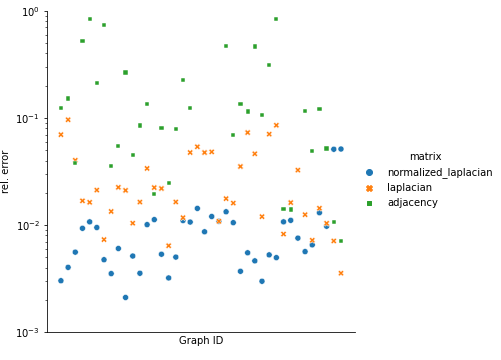
\includegraphics[clip, width=7cm]{./figure/plot_each_graph_k3.png}
            \hspace{1.6cm} k=3
          \end{center}
        \end{minipage}
          % 2
        \begin{minipage}{0.5\hsize}
          \begin{center}
            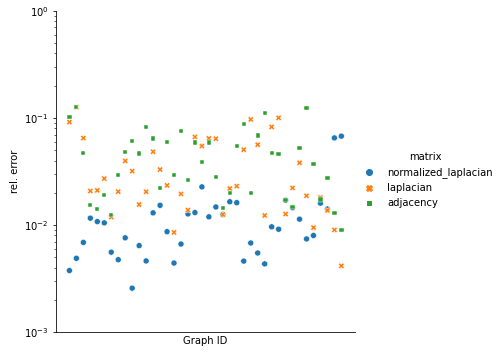
\includegraphics[clip, width=7cm]{./figure/plot_each_graph_k4.png}
            \hspace{1.6cm} k=4
          \end{center}
        \end{minipage}

      \end{tabular}
      \caption{Relative error of SPENet obtained by SQL algorithm.}
      \label{fig:error_each_graph}
    \end{center}
  \end{figure}

We experiment to see how accurately the SQL algorithm can approximate the data. We calculate the SPENet for each of the adjacency matrix, Laplacian matrix, and normalized Laplacian matrix for 40 real-world networks, and illustrate the relative error between the exact values and the values obtained by the SQL algorithm. Figure \ref{fig:error_each_graph} show the results. The detailed values of the relative errors between the exact values of SPENet and the values obtained by the SQL algorithm can be found in Table \ref{tab:rel_error_k3}, \ref{tab:rel_error_k4}.

For the Laplacian and normalized laplacian matrices, the relative error does not change significantly when k is changed. We also conduct experiments with $k = 3.5$ and $4.5$, and the results are similar. However, for the adjacency matrix, the relative error for $k=3$ and $k=4$ differed greatly. This is obviously related to whether ${\mathbf A}^k$ is positive semi-definite or not. For some graphs, the value of the exact solution is 0, and the relative error cannot be defined (Table \ref{tab:rel_error_k3}).

\subsection{Parameter Sensitivity}

\begin{figure}[htbp]
    \begin{center}
      \begin{tabular}{c}
          % 1

        \begin{minipage}{0.33\hsize}
            \begin{center}
              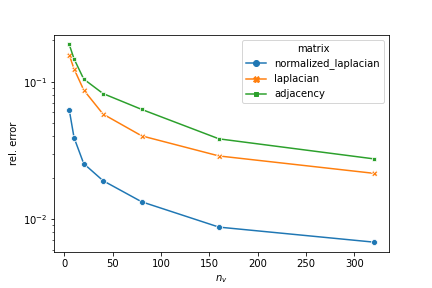
\includegraphics[clip, width=4.5cm]{./figure/plot_param_nv.png}
              \hspace{1.6cm} (a) Number of random starting vectors $n_v$
            \end{center}
        \end{minipage}

        \begin{minipage}{0.33\hsize}
          \begin{center}
            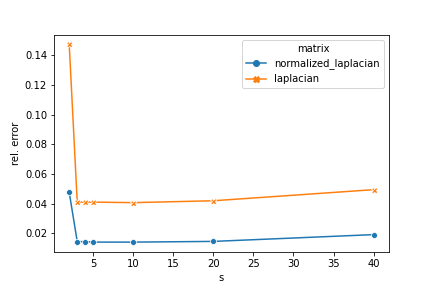
\includegraphics[clip, width=4.5cm]{./figure/plot_param_s.png}
            \hspace{1.6cm} (b) Number of Lanczos iterations $s$
          \end{center}
        \end{minipage}

        \begin{minipage}{0.33\hsize}
          \begin{center}
            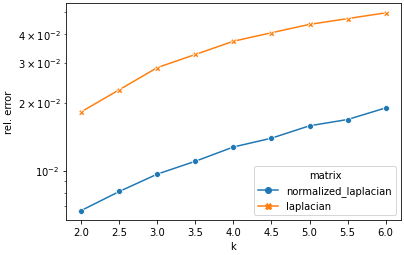
\includegraphics[clip, width=4.5cm]{./figure/plot_param_k.png}
            \hspace{1.6cm} (c) Power $k$
          \end{center}
        \end{minipage}

      \end{tabular}
      \caption{Parameter sensitivity of SLQ algorithm with (a) different number of starting vectors $n_v$, (b) different number of Lanczos iterations $s$ (when $k=4.5$), and (c) different number of power $k$. }
      \label{fig:param_sensitivity}
    \end{center}
  \end{figure}

We investigate how the relative error changes when the parameters change: the number of random starting vectors $n_v$, the step size of the Lanczos algorithm $s$, and power $k$. We calculate the relative error and take the average for 40 real-world networkswith respect to the number of random starting vectors $n_v$, the number of Lanczos iterations $s$ and power $k$ and show the results in the Figure \ref{fig:param_sensitivity}.

There are two sources of error: the stochastic trace estimator and the Gauss quadrature rule. In the experiment in Figure \ref{fig:param_sensitivity}(b), we set $k=4.5$ in order to consider the effect of Lanczos iterations $s$ on the error derived from the Gauss quadrature rule. If $k$ is an integer, the error due to the Gauss quadrature rule becomes 0 when $k \leq 2s-1$. Figure \ref{fig:param_sensitivity}(b) shows that a small value of iterations is sufficient, and the error due to the Gauss quadrature rule is almost negligible if the value is above a certain level. Figure \ref{fig:param_sensitivity}(b) shows that a small value of iterations is sufficient, and the error due to the Gauss quadrature rule is almost negligible for a certain value.


\chapter{Applications and Gallery of Spectral Distributions}
In this chapter, we discuss applications of the spectral distribution defined in Section 2.5. We then show by experiments how the spectral distributions of various synthesized and real-world graphs look in practice.

\section{Quantitative Evaluation and Application}
The DOS and PDOS of a network can be approximated by using the Kernel polynomial method as described in Section 2.5.1. However, its usage has not been discussed in-depth, and only the fact that it can be visualized has been emphasized.
By using this distribution as a discrete probability distribution, it will be possible to evaluate it quantitatively using various concepts such as entropy, divergence, distance.

For each of them, we discuss what advantages and disadvantages they have and compare them with previous studies on similar concepts for networks. As for DOS, even if it becomes possible to evaluate quantitatively by defining entropy, divergence, and distance, similar concepts already exist and can be calculated faster than the method of Kun Dong et al. Therefore, it is not clear at this stage whether there is any advantage in using DOS to evaluate quantitatively.

On the other hand, since there is no similar concept for PDOS, being able to evaluate it quantitatively is a great advantage. In particular, PDOS makes it possible to calculate the distance based on the structure of the network, rather than the shortest distance between vertices.

\subsection{Entropy}
It is possible to calculate the entropy of a spectral distribution expressed as a discrete probability distribution: the entropy of the entire network can be obtained using DOS, and the entropy of each vertex can be obtained using PDOS.

However, Von Neumann graph entropy, a concept similar to the entropy of the entire network, has already been studied \cite{braunstein2006laplacian, chen2019fast,tsitsulin2020just}. It is inspired by the Von Neumann entropy of quantum mechanics and has already been studied not only for applications to divergence and distance but also for applications and properties of the entropy itself. Since there are faster computational methods \cite{chen2019fast,tsitsulin2020just} than those proposed by Kun Dong et al \cite{dong2019network}, there is little advantage in using DOS for entropy .
On the other hand, the entropy per-vertex may be worth using. By considering the relationship between the size of the entropy of each vertex, it may be possible to calculate the "importance" of each vertex.


\subsection{Divergence and Distance}
By using DOS expressed as a discrete probability distribution, it is possible to define the divergence and distance between networks. For example, Kullback-Leibler divergence \cite{kullback1951information} is famous for its divergence, and since Kullback-Leibler divergence is asymmetric, we can also use the symmetric Jeffreys divergence and Jensen-Shannon divergence \cite{nielsen2019jensen, lin1991divergence, jeffreys1946invariant}. It is also possible to use the Jensen-Shannon distance, which was proved to be a valid distance metric \cite{endres2003new}.

The Von Neumann graph entropy can also be used to define divergence and distance, and various studies have already been conducted on this. In the field of quantum mechanics, divergence and quantum Jensen-Shannon divergence have already been defined \cite{briet2009properties, lamberti2008metric}, and these can be calculated using the Von Neumann graph entropy. However, unlike the method of calculating the divergence and distance using DOS, the divergence and distance obtained via Von Neumann graph entropy cannot be precomputed.

However, the distance called NetLSD has also been defined using the heat kernel, and an approximation algorithm has been established \cite{tsitsulin2018netlsd,tsitsulin2020just}. NetLSD is capable of precomputation and can perform approximate calculations faster than DOS. Therefore, when considering the divergence and distance between networks, there is little advantage in using DOS.

On the other hand, there is an advantage of using PDOS. Usually, the distance between vertices is the length of the shortest path, but with this definition, we can express how similar the properties of the vertices are. This may make it possible to search for vertices with similar properties.

\subsection{Applications}
The spectral distribution for networks has not been studied yet, but the spectral distribution for materials has already been studied in the field of condensed matter physics and other fields. It is possible to apply ideas from these fields to networks as well.

For example, a fast online search algorithm for similar spectra has been proposed \cite{borysov2018online,geilhufe2018towards}, and since DOS and PDOS are capable of precomputation, the results of the calculation can be stored in a database for fast search of networks with similar spectra. In this case, it is necessary to define the distance between two networks, which can be expressed as a vector by considering DOS as a discrete distribution, and Euclidean distance and cosine distance can be used.

\section{Experiments}
\subsection{Gallery of DOS/PDOS}
We show the results of DOS and PDOS for synthesized graphs and real-world networks. We use the method proposed by Kun Dong et al. based on the kernel polynomial method (KMP) as described in Section 2.5.1. motif filtering is not used, and the perturbations are smoothed using Jackson damping after calculation using the kernel polynomial method. The perturbations are smoothed using Jackson damping.

If there is a spike in the spectral distribution of the DOS, we zoom in on the DOS so that we can see the lower shape. The red dots mean the values obtained by the KMP-based approximation.
The PDOS computed for all vertices are sorted and then displayed vertically. Red means that the weight of a part of the spectrum of a vertex is large, while blue means that the weight is small.

\subsubsection*{Parameter Settings.}
Unless otherwise stated, we use 1000 Chebyshev moments, 20 random vectors, and 51 histogram bins in our experiments.

\subsubsection*{Datasets.}
% ~の sythesized Graph と、 ~のreal world graph に対して実験する。


\subsubsection{Synthesized Graph}


\subsubsection{Real-World Network}

\subsection{Propaties of Graphs with Similar DOS/PDOS}
Motif multiplicity corresponds to eigenvalues multiplicity \cite{mehatari2015effect,dong2019network}.


\chapter{Conclusion}
We discussed how to use all the eigenvalues of a large network for analysis and application.

First, we proposed the STE algorithm and the SLQ algorithm as algorithms for approximating the sum of the powers of the eigenvalues. These algorithms are the first algorithms for finding SPEs that scale to large graphs. For the Laplacian and normalized Laplacian matrices, good approximations were obtained in most of the experimental cases. For the Laplacian and normalized Laplacian matrices, good approximations were obtained in most experimental cases.

However, when k is an odd number, we found experimentally that the algorithm does not work well for adjacency matrices, such as bipartite graphs or matrices with many closed paths. k is 3, it can be obtained by triangle counting, so it may be better to use another approximation algorithm. In the case of k = 3, it is possible to obtain the result by triangle counting, so it may be better to use another approximation algorithm. There are several types of starting random vectors, and the error bound that can be given depends on which one is chosen. There are some previous studies on the errors generated by stochastic trace estimators, but they do not become positive semi-definite when applied to adjacency matrices with k odd. Also, there is no mention of the error caused by the Gauss quadrature rule when k is a real number. The error bound and variance for these are open problems.


Next, the DOS and PDOS of large-scale networks that can be obtained by using the Kernel Polynomial Method are discussed. Although previous studies have shown that the visualization of these values is a great advantage, the specific use of these values is not described in detail. We discussed that for PDOS, quantitative evaluation could be a new evaluation index that would allow comparison among vertices. We also calculated and showed DOS and PDOS for synthesized graphs and real-world networks where the spectral distribution is not yet known. As a result, it can be inferred that networks with a common spectrum would have common properties. This provides a stepping stone for the analysis of networks using spectral distribution.

However, we have not been able to show what the distance between vertices using PDOS means in concrete terms. If we can show some results even experimentally, it will be a clue for the future. Also, the correspondence between the spectral distribution and the nature of the network is only inferred and not formally discussed. It is well known that a random graph has a semicircular spectrum, but it is necessary to show how other shapes correspond to the properties of the network.

\subsection*{Future research}
To take the analysis of large-scale graphs to the next stage, where only some eigenvalues have been used, it is necessary to conduct research using all eigenvalues.

The following should be done for the sum of powers of eigenvalues.
\begin{itemize}
    \item To show the error bounds of the STE/SLQ algorithm.
    \item To show under what conditions the algorithm does not compute well when k is odd and applied to an adjacency matrix.
\end{itemize}

For DOS and PDOS, the following are desired
\begin{itemize}
    \item To show what other applications are possible by quantitative evaluation of DOS and PDOS.
    \item To show the meaning of the distance between vertices using PDOS.
    \item To show the correspondence between the spectral distribution and the properties of the network.
\end{itemize}


%-------------------
\bibliographystyle{plain} % 参考文献
\bibliography{myref} %
%-------------------

\appendix
\chapter{Data Source and Characteristics}
\begin{table}[htb]
    \begin{center}
      \scalebox{0.75}{
      \begin{tabular}{l | c c c c c}
        Graph & $|V|$ & $|E|$ & AVg. deg. & Density & weighted/unweighted  \\ \hline
        bio-celegans & 453 & 2025 & 8.94 & 9.89e-03 & unweighted\\
        bio-celegans-dir & 453 & 2040 & 9.01 & 9.96e-03 & unweighted\\
        bio-diseasome & 516 & 1188 & 4.60 & 4.47e-03 & unweighted\\
        ENZYMES\_g295 & 123 & 139 & 2.26 & 9.26e-03 & unweighted\\
        ENZYMES\_g296 & 125 & 141 & 2.26 & 9.10e-03 & unweighted\\
        ENZYMES\_g297 & 121 & 149 & 2.46 & 1.03e-02 & unweighted\\
        ia-crime-moreno & 829 & 1475 & 3.56 & 2.15e-03 & unweighted\\
        ia-email-univ & 1133 & 5451 & 9.62 & 4.25e-03 & unweighted\\
        ia-enron-only & 143 & 623 & 8.71 & 3.07e-02 & unweighted\\
        ia-fb-messages & 1266 & 6451 & 10.19 & 4.03e-03 & unweighted\\
        ia-infect-dublin & 410 & 2765 & 13.49 & 1.65e-02 & unweighted\\
        ia-infect-hyper & 113 & 2196 & 38.87 & 1.74e-01 & unweighted\\
        adjnoun & 112 & 425 & 7.59 & 3.42e-02 & unweighted\\
        bcspwr03 & 118 & 297 & 5.03 & 2.15e-02 & unweighted\\
        bibd\_9\_5 & 126 & 1217 & 19.32 & 7.73e-02 & unweighted\\
        can\_144 & 144 & 720 & 10.00 & 3.50e-02 & unweighted\\
        polbooks & 105 & 441 & 8.40 & 4.04e-02 & unweighted\\
        flower\_4\_1 & 129 & 380 & 5.89 & 2.30e-02 & unweighted\\
        fs-adjnoun\_adj\_copperfield & 112 & 425 & 7.59 & 3.42e-02 & unweighted\\
        GD06\_theory & 101 & 190 & 3.76 & 1.88e-02 & unweighted\\
        GD96\_b & 111 & 193 & 3.48 & 1.58e-02 & unweighted\\
        GD98\_b & 121 & 132 & 2.18 & 9.09e-03 & unweighted\\
        GD98\_c & 112 & 168 & 3.00 & 1.35e-02 & unweighted\\
        GD99\_c & 105 & 120 & 2.29 & 1.10e-02 & unweighted\\
        gent113 & 113 & 639 & 11.31 & 5.05e-02 & unweighted\\
        bio-CE-GT & 924 & 3239 & 7.01 & 3.80e-03 & weighted\\
        bio-CE-LC & 1387 & 1648 & 2.38 & 8.57e-04 & weighted\\
        bio-DM-LC & 658 & 1129 & 3.43 & 2.61e-03 & weighted\\
        bio-SC-TS & 636 & 3959 & 12.45 & 9.80e-03 & weighted\\
        eco-florida & 128 & 2075 & 32.42 & 1.28e-01 & weighted\\
        eco-foodweb-baydry & 128 & 2106 & 32.91 & 1.30e-01 & weighted\\
        gre\_115 & 115 & 382 & 6.64 & 2.91e-02 & weighted\\
        gre\_185 & 185 & 835 & 9.03 & 2.45e-02 & weighted\\
        IG5-7 & 136 & 549 & 8.07 & 2.99e-02 & weighted\\
        jazz & 198 & 2742 & 27.70 & 7.03e-02 & weighted\\
        misc-football & 115 & 612 & 10.64 & 4.67e-02 & weighted\\
        rw136 & 136 & 373 & 5.49 & 2.03e-02 & weighted\\
        TF10 & 107 & 579 & 10.82 & 5.10e-02 & weighted\\
        Trefethen\_150 & 150 & 1095 & 14.60 & 4.90e-02 & weighted\\
        Trefethen\_200b & 199 & 1536 & 15.44 & 3.90e-02 & weighted\\
      \end{tabular}
      }
      \caption{Characteristics of 40 small real-world networks used in Chapter 3 which come from NETWORK REPOSITORY; number of vertices $|V|$, number of edges $|E|$, average node degree, density of graph $|E|/ \binom{|V|}{2}$, weighted or unweighted graph}
      \label{tab:data_spe}
    \end{center}
  \end{table}

\chapter{Detailed Experimental Results on SPENet}

\begin{table}[htb]
    \begin{center}
      \scalebox{0.80}{
      \begin{tabular}{l | c c | c c | c c }
             & \multicolumn{2}{c}{${\mathbf A}$} & \multicolumn{2}{c}{${\mathbf L}$} & \multicolumn{2}{c}{${\mathbfcal L}$} \\
        Graph & exact & rel. error & exact & rel. error & exact & rel. error  \\ \hline
        bio-celegans & 1.970e+04 & 0.12352 & 2.106e+07 & 0.06977 & 5.931e+02 & 0.00302\\
        bio-celegans-dir & 2.130e+04 & 0.15158 & 2.106e+07 & 0.09613 & 5.825e+02 & 0.00403\\
        bio-diseasome & 8.160e+03 & 0.03805 & 4.305e+05 & 0.04023 & 8.243e+02 & 0.00559\\
        ENZYMES\_g295 & 1.200e+01 & 0.51855 & 4.238e+03 & 0.01685 & 2.880e+02 & 0.00933\\
        ENZYMES\_g296 & 1.200e+01 & 0.83381 & 4.050e+03 & 0.01630 & 2.931e+02 & 0.01071\\
        ENZYMES\_g297 & 5.400e+01 & 0.21166 & 5.458e+03 & 0.02121 & 2.710e+02 & 0.00949\\
        ia-crime-moreno & 1.640e+02 & 0.73894 & 2.284e+05 & 0.00732 & 1.431e+03 & 0.00475\\
        ia-email-univ & 3.206e+04 & 0.03573 & 6.076e+06 & 0.01340 & 1.496e+03 & 0.00352\\
        ia-enron-only & 5.334e+03 & 0.05443 & 3.260e+05 & 0.02250 & 1.929e+02 & 0.00604\\
        ia-fb-messages & 1.495e+04 & 0.26510 & 1.793e+07 & 0.02107 & 1.644e+03 & 0.00211\\
        ia-infect-dublin & 4.268e+04 & 0.04542 & 2.653e+06 & 0.01041 & 5.074e+02 & 0.00514\\
        ia-infect-hyper & 1.012e+05 & 0.08505 & 1.201e+07 & 0.01640 & 1.204e+02 & 0.00355\\
        adjnoun & 1.704e+03 & 0.13554 & 3.067e+05 & 0.03379 & 1.532e+02 & 0.01010\\
        bcspwr03 & 1.330e+03 & 0.01962 & 1.052e+04 & 0.02238 & 8.858e+01 & 0.01124\\
        bibd\_9\_5 & 1.734e+04 & 0.08087 & 2.941e+06 & 0.02195 & 1.379e+02 & 0.00534\\
        can\_144 & 9.072e+03 & 0.02465 & 1.348e+05 & 0.00642 & 1.274e+02 & 0.00321\\
        polbooks & 3.360e+03 & 0.07925 & 1.942e+05 & 0.01643 & 1.388e+02 & 0.00502\\
        flower\_4\_1 & 2.960e+02 & 0.22451 & 4.469e+04 & 0.01172 & 1.888e+02 & 0.01103\\
        fs-adjnoun\_adj\_copperfield & 1.704e+03 & 0.12304 & 3.067e+05 & 0.04755 & 1.532e+02 & 0.01067\\
        GD06\_theory & 0.000e+00 & inf & 8.252e+04 & 0.05384 & 1.297e+02 & 0.01430\\
        GD96\_b & 0.000e+00 & inf & 1.705e+05 & 0.04754 & 1.643e+02 & 0.00865\\
        GD98\_b & 0.000e+00 & inf & 9.006e+03 & 0.04821 & 2.525e+02 & 0.01202\\
        GD98\_c & 0.000e+00 & inf & 6.048e+03 & 0.01085 & 2.240e+02 & 0.01085\\
        GD99\_c & 1.200e+01 & 0.47025 & 4.188e+03 & 0.01764 & 2.336e+02 & 0.01331\\
        gent113 & 5.718e+03 & 0.06876 & 2.759e+05 & 0.01604 & 9.869e+01 & 0.01053\\
        bio-CE-GT & 2.892e+05 & 0.13453 & 1.462e+08 & 0.03521 & 1.247e+03 & 0.00370\\
        bio-CE-LC & 2.756e+04 & 0.11485 & 1.754e+07 & 0.07303 & 2.628e+03 & 0.00551\\
        bio-DM-LC & 4.865e+04 & 0.46453 & 2.852e+07 & 0.04627 & 1.338e+03 & 0.00463\\
        bio-SC-TS & 1.211e+07 & 0.10717 & 8.366e+08 & 0.01198 & 1.149e+03 & 0.00299\\
        eco-florida & 5.750e+07 & 0.31274 & 3.990e+09 & 0.07063 & 1.410e+02 & 0.00527\\
        eco-foodweb-baydry & 1.343e+07 & 0.83741 & 1.751e+09 & 0.08539 & 1.406e+02 & 0.00497\\
        gre\_115 & 6.026e+01 & 0.01424 & 1.452e+02 & 0.00824 & 5.337e+01 & 0.01071\\
        gre\_185 & 5.860e+01 & 0.01398 & 3.152e+02 & 0.01621 & 1.511e+02 & 0.01107\\
        IG5-7 & 0.000e+00 & inf & 2.173e+06 & 0.03258 & 1.826e+02 & 0.00755\\
        jazz & 8.592e+05 & 0.11688 & 8.523e+07 & 0.01249 & 2.221e+02 & 0.00566\\
        misc-football & 4.920e+03 & 0.04891 & 1.789e+05 & 0.00721 & 1.437e+02 & 0.00653\\
        rw136 & 1.689e+01 & 0.12035 & 7.461e+02 & 0.01435 & 2.336e+02 & 0.01304\\
        TF10 & 1.132e+04 & 0.05180 & 6.611e+05 & 0.01038 & 1.382e+02 & 0.00976\\
        Trefethen\_150 & 2.164e+10 & 0.01076 & 3.739e+05 & 0.00711 & 2.241e+00 & 0.05102\\
        Trefethen\_200b & 8.051e+10 & 0.00708 & 5.962e+05 & 0.00356 & 1.553e+00 & 0.05127\\
      \end{tabular}
      }
      \caption{The relative error between the exact value of SPENet and the value obtained by the SLQ algorithm when $k=3$, $Nv = 100$, $s= 10$. The relative error is the average of 10 results.}
      \label{tab:rel_error_k3}
    \end{center}
  \end{table}


\begin{table}[htb]
    \begin{center}
      \scalebox{0.80}{
      \begin{tabular}{l | c c | c c | c c }
             & \multicolumn{2}{c}{${\mathbf A}$} & \multicolumn{2}{c}{${\mathbf L}$} & \multicolumn{2}{c}{${\mathbfcal L}$} \\
        Graph & exact & rel. error & exact & rel. error & exact & rel. error  \\ \hline
        bio-celegans & 7.231e+05 & 0.10165 & 3.903e+09 & 0.09142 & 7.305e+02 & 0.00376\\
        bio-celegans-dir & 7.400e+05 & 0.12676 & 3.903e+09 & 0.12592 & 7.121e+02 & 0.00490\\
        bio-diseasome & 8.139e+04 & 0.04701 & 1.251e+07 & 0.06481 & 1.128e+03 & 0.00689\\
        ENZYMES\_g295 & 1.162e+03 & 0.01531 & 2.045e+04 & 0.02080 & 4.911e+02 & 0.01160\\
        ENZYMES\_g296 & 1.150e+03 & 0.01407 & 1.869e+04 & 0.02107 & 5.004e+02 & 0.01078\\
        ENZYMES\_g297 & 1.450e+03 & 0.01923 & 2.962e+04 & 0.02715 & 4.530e+02 & 0.01049\\
        ia-crime-moreno & 3.480e+04 & 0.01244 & 3.337e+06 & 0.01188 & 2.127e+03 & 0.00558\\
        ia-email-univ & 7.453e+05 & 0.02937 & 2.157e+08 & 0.02051 & 1.873e+03 & 0.00475\\
        ia-enron-only & 7.669e+04 & 0.04794 & 7.964e+06 & 0.03969 & 2.428e+02 & 0.00760\\
        ia-fb-messages & 1.218e+06 & 0.06120 & 1.188e+09 & 0.03189 & 2.050e+03 & 0.00258\\
        ia-infect-dublin & 8.518e+05 & 0.04651 & 7.534e+07 & 0.01554 & 5.974e+02 & 0.00643\\
        ia-infect-hyper & 4.883e+06 & 0.08284 & 7.556e+08 & 0.02045 & 1.269e+02 & 0.00463\\
        adjnoun & 4.320e+04 & 0.06417 & 1.046e+07 & 0.04831 & 1.971e+02 & 0.01300\\
        bcspwr03 & 5.436e+03 & 0.02216 & 7.290e+04 & 0.03299 & 1.020e+02 & 0.01529\\
        bibd\_9\_5 & 6.324e+05 & 0.05986 & 1.257e+08 & 0.02347 & 1.507e+02 & 0.00868\\
        can\_144 & 7.646e+04 & 0.02932 & 1.709e+06 & 0.00855 & 1.329e+02 & 0.00442\\
        polbooks & 4.824e+04 & 0.07557 & 3.853e+06 & 0.01953 & 1.708e+02 & 0.00665\\
        flower\_4\_1 & 9.484e+03 & 0.02650 & 4.010e+05 & 0.01381 & 2.562e+02 & 0.01270\\
        fs-adjnoun\_adj\_copperfield & 4.320e+04 & 0.05895 & 1.046e+07 & 0.06645 & 1.971e+02 & 0.01309\\
        GD06\_theory & 8.840e+03 & 0.03902 & 1.640e+06 & 0.05468 & 1.637e+02 & 0.02272\\
        GD96\_b & 1.443e+04 & 0.05902 & 7.043e+06 & 0.06453 & 2.303e+02 & 0.01194\\
        GD98\_b & 1.812e+03 & 0.02810 & 7.851e+04 & 0.06398 & 4.118e+02 & 0.01475\\
        GD98\_c & 1.680e+03 & 0.01447 & 2.890e+04 & 0.01255 & 3.567e+02 & 0.01255\\
        GD99\_c & 1.136e+03 & 0.01994 & 2.102e+04 & 0.02195 & 3.913e+02 & 0.01650\\
        gent113 & 1.087e+05 & 0.05440 & 5.333e+06 & 0.02310 & 1.090e+02 & 0.01618\\
        bio-CE-GT & 2.126e+07 & 0.08734 & 3.670e+10 & 0.05054 & 1.564e+03 & 0.00461\\
        bio-CE-LC & 2.606e+06 & 0.02000 & 2.345e+09 & 0.09681 & 4.175e+03 & 0.00680\\
        bio-DM-LC & 1.866e+07 & 0.06872 & 3.716e+09 & 0.05626 & 2.186e+03 & 0.00549\\
        bio-SC-TS & 2.650e+09 & 0.11070 & 1.870e+11 & 0.01229 & 1.767e+03 & 0.00434\\
        eco-florida & 1.564e+11 & 0.04700 & 4.221e+12 & 0.08246 & 1.552e+02 & 0.00962\\
        eco-foodweb-baydry & 6.110e+10 & 0.04625 & 1.553e+12 & 0.10027 & 1.546e+02 & 0.00915\\
        gre\_115 & 6.711e+01 & 0.01706 & 2.164e+02 & 0.01267 & 5.662e+01 & 0.01705\\
        gre\_185 & 7.057e+01 & 0.01469 & 5.120e+02 & 0.02223 & 1.845e+02 & 0.01453\\
        IG5-7 & 1.894e+06 & 0.05269 & 1.275e+08 & 0.03817 & 2.348e+02 & 0.01136\\
        jazz & 5.872e+07 & 0.12467 & 9.929e+09 & 0.01878 & 2.431e+02 & 0.00742\\
        misc-football & 5.780e+04 & 0.03688 & 2.280e+06 & 0.00948 & 1.688e+02 & 0.00799\\
        rw136 & 8.680e+01 & 0.01732 & 1.652e+03 & 0.01809 & 3.390e+02 & 0.01601\\
        TF10 & 3.425e+05 & 0.02770 & 1.518e+07 & 0.01370 & 1.752e+02 & 0.01412\\
        Trefethen\_150 & 1.498e+13 & 0.01296 & 5.616e+06 & 0.00902 & 1.561e+00 & 0.06509\\
        Trefethen\_200b & 7.826e+13 & 0.00896 & 9.494e+06 & 0.00417 & 9.466e-01 & 0.06762\\
      \end{tabular}
      }
      \caption{The relative error between the exact value of SPENet and the value obtained by the SLQ algorithm when $k=4$, $Nv = 100$, $s= 10$. The relative error is the average of 10 results.}
      \label{tab:rel_error_k4}
    \end{center}
  \end{table}


\end{document}
